\documentclass[a4paper, 12pt]{article}
\usepackage[top=1.8cm, bottom=1.8cm, left=1.5cm, right=1.5cm]{geometry}
\usepackage[utf8]{inputenc}
\usepackage{amsmath}
\usepackage{graphicx}

\begin{document}
	\begin{center}
		Universidade Federal do Rio Grande do Norte
		
		Departamento de Engenharia da Computação e Automação  
		
		DCA3703 - Programação Paralela  
		
		\textbf{Tarefa 11: Impacto das cláusulas schedule e collapse}  
		
		\textbf{Aluno:} Daniel Bruno Trindade da Silva  
	\end{center}  
	
	\section{Introdução}  
	\hspace{.62cm}Este relatório tem como objetivo apresentar o conhecimento adquirido durante a realização da Tarefa 11 da disciplina de \textbf{Computação Paralela}. A atividade consistiu em um estudo voltado à fixação dos conceitos relacionados às cláusulas \texttt{schedule} e \texttt{collapse}, bem como à análise de seus impactos em códigos paralelizados utilizando a biblioteca \textbf{OpenMP}.  
	
	\section{Enunciado}   
	
	\hspace{.62cm}Escreva um código que simule o movimento de um fluido ao longo do tempo usando a equação de Navier-Stokes, considerando apenas os efeitos da viscosidade. Desconsidere a pressão e quaisquer forças externas. Utilize diferenças finitas para discretizar o espaço e simule a evolução da velocidade do fluido no tempo. Inicialize o fluido parado ou com velocidade constante e verifique se o campo permanece estável. Em seguida, crie uma pequena perturbação e observe se ela se difunde suavemente. Após validar o código, paralelize-o com OpenMP e explore o impacto das cláusulas schedule e collapse no desempenho da execução paralela.  
	
	\section{Desenvolvimento}  
	\hspace{.62cm}Como solicitado no enunciado, foi criado um código para a implementação da simulação da velocidade do fluido. O fluido foi representado como uma matriz tridimensional de velocidades, discretizada em uma malha de dimensões \( NX \times NY \times NZ = 20 \times 20 \times 20 \), com espaçamento \( \Delta x = \Delta y = \Delta z = 0.01 \). A equação de Navier-Stokes foi simplificada, considerando apenas o termo de viscosidade:  
	
	\[  
	\frac{\partial \mathbf{u}}{\partial t} = \nu \nabla^2 \mathbf{u},  
	\]  
	onde \( \nu \) é a viscosidade cinemática (\( \nu = 0.01 \)) e \( \nabla^2 \) é o Laplaciano.  
	
	\subsection{Implementação do Código}  
	A discretização utilizou o método de diferenças finitas:  
	\begin{itemize}  
		\item \textbf{Condições Iniciais}: O campo de velocidade foi inicializado com valores nulos, exceto no centro do domínio, onde uma perturbação de magnitude 1 foi inserida.
		
		\begin{verbatim}
			void initialize(double u[NX][NY][NZ]) {
				for (int i = 0; i < NX; i++) {
					for (int j = 0; j < NY; j++) {
						for (int k = 0; k < NZ; k++) {
							u[i][j][k] = 0.0;
						}
					}
				}
				int cx = NX / 2;
				int cy = NY / 2;
				int cz = NZ / 2;
				u[cx][cy][cz] = 1.0;
			}
		\end{verbatim}
		  
		\item \textbf{Condições de Contorno}: Velocidade fixa (\( u = 0 \)) em todas as bordas do domínio.
		
		\begin{verbatim}
			void apply_boundary_conditions(double u[NX][NY][NZ]) {
				for (int i = 0; i < NX; i++) {
					for (int j = 0; j < NY; j++) {
						u[i][j][0] = 0.0;
						u[i][j][NZ-1] = 0.0;
					}
					for (int k = 0; k < NZ; k++) {
						u[i][0][k] = 0.0;
						u[i][NY-1][k] = 0.0;
					}
				}
				for (int j = 0; j < NY; j++) {
					for (int k = 0; k < NZ; k++) {
						u[0][j][k] = 0.0;
						u[NX-1][j][k] = 0.0;
					}
				}
			}
		\end{verbatim}
		
		\item \textbf{Atualização Temporal}: O Laplaciano foi calculado para cada ponto interno da malha, utilizando diferenças centradas. O passo de tempo (\( \Delta t = 10^{-5} \)) garantiu estabilidade numérica. 
		
		\begin{verbatim}
			void update(double u[NX][NY][NZ], double u_new[NX][NY][NZ]) {
				for (int i = 1; i < NX-1; i++) {
					for (int j = 1; j < NY-1; j++) {
						for (int k = 1; k < NZ-1; k++) {
							double dudx2 = (u[i+1][j][k] - 2*u[i][j][k] + u[i-1][j][k]) / (DX*DX);
							double dudy2 = (u[i][j+1][k] - 2*u[i][j][k] + u[i][j-1][k]) / (DY*DY);
							double dudz2 = (u[i][j][k+1] - 2*u[i][j][k] + u[i][j][k-1]) / (DZ*DZ);
							u_new[i][j][k] = u[i][j][k] + NU * DT * (dudx2 + dudy2 + dudz2);
						}
					}
				}
			}
		\end{verbatim}
		 
	\end{itemize}  
	
	\subsection{Validação}  
		\hspace{.62cm}Inicialmente, verificou-se a estabilidade do campo sem perturbações. Posteriormente, a introdução da perturbação no centro resultou em uma difusão suave, conforme esperado para um fluido viscoso. A evolução da velocidade no centro (\( u_{\text{centro}} \)) foi monitorada a cada 50 passos, exibindo um decaimento gradual.  
	
	\begin{figure}[h]
		\centering
		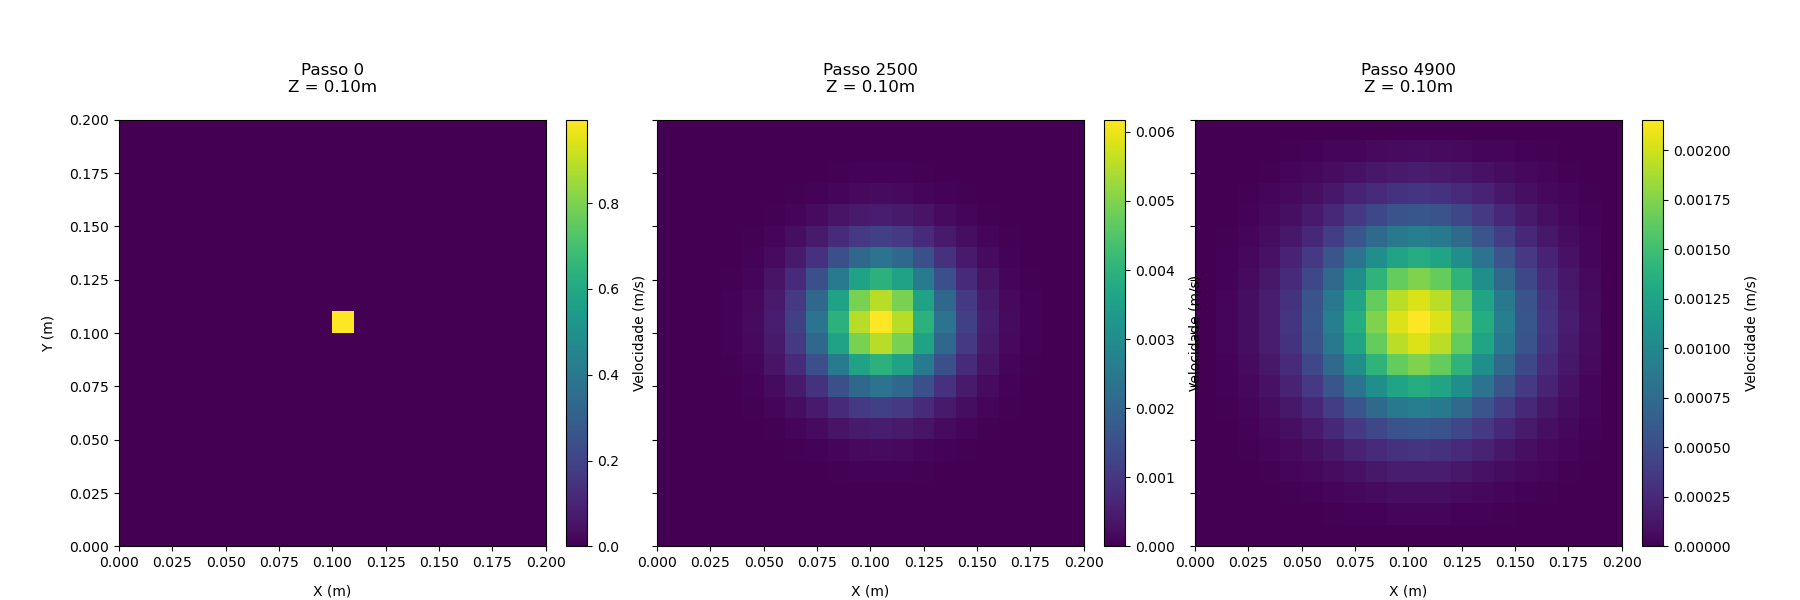
\includegraphics[width=\linewidth]{imgs/Figure_1.png}
		\caption{Difusão da perturbação inicial nos passos 0 (início), 2500 (meio) e 4900 (fim) da simulação. A escala de cores representa a magnitude da velocidade.}
	\end{figure}
	
	\subsection{Paralelização com OpenMP}  
	O código foi paralelizado utilizando as seguintes estratégias:  
	\begin{itemize}  
		\item \textbf{Collapse}: A cláusula \texttt{collapse(3)} foi aplicada em loops aninhados para "achatar" a iteração tridimensional, aumentando o grau de paralelismo.  
		\item \textbf{Schedule}: Foram testadas as políticas \texttt{static}, \texttt{dynamic}, \texttt{guided} e \texttt{auto}, com diferentes números de threads e de \textit{chunk}.  
		\item \textbf{Regiões Críticas}: As funções \texttt{initialize}, \texttt{apply\_boundary\_conditions} e \texttt{update} foram paralelizadas, utilizando o \texttt{colapse} e \texttt{schedule}. 
	\end{itemize}  
	
	\subsection{Análise de Desempenho}  
		\hspace{.62cm}Para comparar o desempenho da aplicação das configurações da cláusula \texttt{schedule}, variamos os parâmetros (\texttt{static}, \texttt{dynamic}, \texttt{guided} e \texttt{auto}) e o número de threads (1, 2, 4 e 8) em nossos testes e estes são os resultados obtidos:
	
	\begin{table}[htbp]
		\centering
		\caption{Comparação de desempenho entre configurações de schedule OpenMP (tempo em segundos)}
		
		\vspace{1cm}
		\begin{tabular}{|c|c|c|c|c|}
			\hline
			\textbf{Threads} & \textbf{Static} & \textbf{Dynamic (4)} & \textbf{Guided} & \textbf{Auto} \\
			\hline
			1 & 10.596022 & 12.877296 & 10.612986 & 10.582557 \\
			\hline
			2 & 5.880238 & 8.701045 & 5.841041 & 5.826200 \\
			\hline
			4 & 3.559344 & 5.797681 & 3.514549 & 3.546131 \\
			\hline
			8 & 3.385047 & 5.076297 & 3.595373 & 3.433562 \\
			\hline
		\end{tabular}
		\label{tab:openmp_schedule_performance}
	\end{table}  
	
	Esses testes foram executados em um computador com 16Gb de memória e com processador i3 10100f com 4 núcleos sendo 2 threads por núcleo. 
	
	Analisando os resultados temos:
	
	\begin{itemize}  
		\item \texttt{static}: Teve um bom desempenho devido ao fato de que o problema é homogêneo, ou seja, suas iterações são balanceadas e com cálculos regulares;
		\item \texttt{dynamic}: Apresentou o pior desempenho devido ao \textit{overhead} de gerenciamento. Testes com chunk maior melhoraram o desempenho em cerca de 1s, mas ainda inferior às demais políticas. Essa configuração é mais adequada para cargas desbalanceadas;
		\item \texttt{guided}: Teve desempenho muito próximo ao \texttt{static}, e seria vantajosa em casos com maior variação de carga, dado seu bom balanceamento com baixo \textit{overhead};
		\item \texttt{auto}: Teve desempenho similar ao \texttt{static}, sugerindo que o runtime escolheu essa estratégia internamente.
	\end{itemize}  
	
	\section{Conclusão}  
	\hspace{.62cm}A realização da Tarefa 11 permitiu consolidar conceitos fundamentais da programação paralela utilizando a biblioteca OpenMP, com foco nas cláusulas \texttt{collapse} e \texttt{schedule}. Observou-se que a utilização de \texttt{collapse(3)} foi essencial para aumentar o grau de paralelismo ao distribuir eficientemente as iterações dos loops aninhados em três dimensões.  
	
	Em relação à cláusula \texttt{schedule}, os testes demonstraram que a política \texttt{static} teve o melhor desempenho geral, especialmente com 4 e 8 threads, devido à natureza homogênea da carga de trabalho. A política \texttt{dynamic}, por outro lado, apresentou desempenho inferior devido ao alto overhead de gerenciamento, pouco vantajoso em um problema com iterações balanceadas. Já a política \texttt{guided} apresentou desempenho competitivo, indicando potencial em contextos com maior variabilidade de carga. A opção \texttt{auto} mostrou desempenho semelhante ao \texttt{static}, o que sugere que o compilador identificou corretamente a melhor estratégia para o cenário.
	
	Com isso, conclui-se que a escolha adequada de estratégias de paralelização tem impacto direto no desempenho de aplicações paralelas. O domínio das cláusulas \texttt{schedule} e \texttt{collapse} é essencial para maximizar o aproveitamento dos recursos computacionais, especialmente em simulações científicas com grandes volumes de dados. Esta tarefa proporcionou uma experiência prática valiosa, permitindo observar na prática como diferentes abordagens afetam o desempenho e a escalabilidade do código.
\end{document}
